\tikzstyle{area} = [rectangle,draw,minimum height=3cm,minimum width=2cm]
\tikzstyle{assembly} = [rectangle,draw,minimum height=0.75cm,minimum width=0.5cm]
\tikzstyle{every node}=[font=\LARGE]
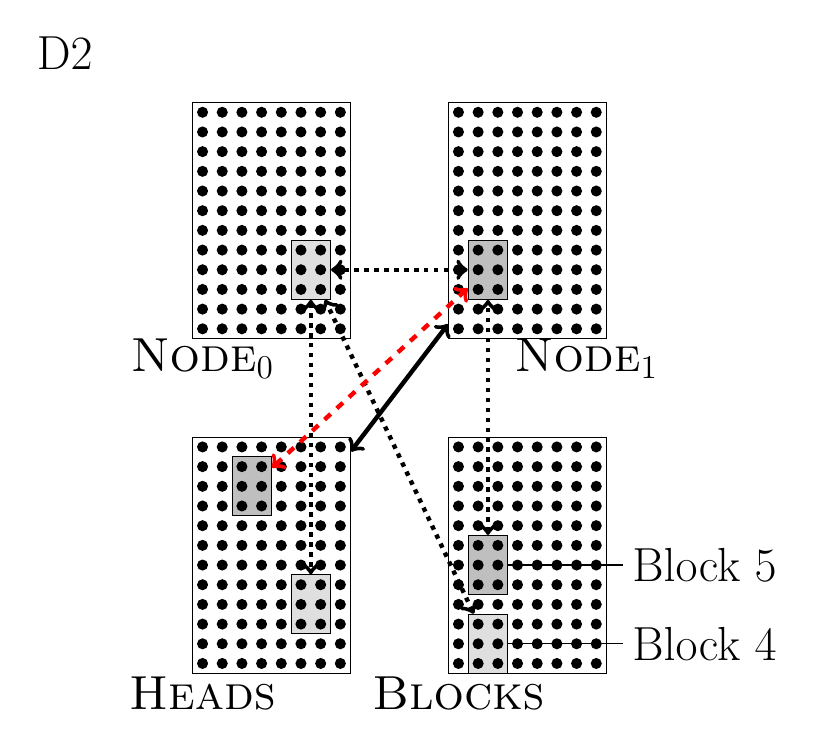
\begin{tikzpicture}[x=0.25cm,y=0.25cm]
	\node[area] (B) at (3.5,5.5) {};
	\node at (0,-1.5) {\textsc{Blocks}};
	\node[assembly,fill=gray!25] (b1) at (1.5,1) {};
	\node[align=left] (b1t) at (12.5,1) {Block $4$};
	\node[assembly,fill=gray!50] (b2) at (1.5,5) {};
	\node[align=left] (b2t) at (12.5,5) {Block $5$};
	\foreach \x in {0,...,7}
	\foreach \y in {0,...,11}
	{\fill (\x,\y) circle (2pt);}
	\draw (b1) -- (b1t);
	\draw (b2) -- (b2t);
	\begin{scope}[xshift=-3.25cm,yshift=4.25cm]
		\node[area] (N1) at (3.5,5.5) {};
		\node at (0,-1.5) {\mbox{\textsc{Node}$_0$}};
		\node[assembly,fill=gray!25] (n1) at (5.5,3) {};
		\foreach \x in {0,...,7}
		\foreach \y in {0,...,11}
		{\fill (\x,\y) circle (2pt);}
		\draw[<->,ultra thick,dotted] (b1) -- (n1);
	\end{scope}
	\begin{scope}[xshift=0cm,yshift=4.25cm]
		\node[area] (N2) at (3.5,5.5) {};
		\node at (6.5,-1.5) {\mbox{\textsc{Node}$_1$}};
		\node[assembly,fill=gray!50] (n2) at (1.5,3) {};
		\foreach \x in {0,...,7}
		\foreach \y in {0,...,11}
		{\fill (\x,\y) circle (2pt);}
		\draw[<->,ultra thick,dotted] (b2) -- (n2);
		\draw[<->,ultra thick,dotted] (n1) -- (n2);
	\end{scope}
	\begin{scope}[xshift=-3.25cm,yshift=0cm]
		\node[area] (H) at (3.5,5.5) {};
		\node at (0,-1.5) {\textsc{Heads}};
		\node[assembly,fill=gray!25] (h) at (5.5,3) {};
		\node[assembly,fill=gray!50] (nh) at (2.5,9) {};
		\foreach \x in {0,...,7}
		\foreach \y in {0,...,11}
		{\fill (\x,\y) circle (2pt);}
		\draw[<->,ultra thick] (H) -- (N2);
		\draw[<->,ultra thick,dotted] (n1) -- (h);
		\draw[<->,ultra thick,color=red,dashed] (n2) -- (nh);
	\end{scope}
	\node at (-20,31) {\LARGE D2};
\end{tikzpicture}